% Lab 4 report - CO3009 Microprocessors - Microcontrollers
% Build: xelatex (run twice)
\documentclass[12pt,a4paper]{article}

% ------------------------------------------------------------------
% Video link: put the real URL between the braces, e.g.
% \newcommand{\videolink}{https://drive.google.com/file/d/xxxx/view}
% Leave it empty and the video paragraph is left out of the PDF.
\newcommand{\videolink}{}
% ------------------------------------------------------------------

\usepackage{fontspec}
\setmainfont{Latin Modern Roman}
\setmonofont{Latin Modern Mono}[Scale=0.95]
\usepackage[a4paper,left=2.5cm,right=2.2cm,top=2.8cm,bottom=2.5cm,headheight=34pt]{geometry}
\usepackage{graphicx,xcolor,booktabs,tabularx,array,float,enumitem,amsmath,etoolbox}
\usepackage[font=small,labelfont=rm]{caption}
\usepackage{listings}
\usepackage{multirow}
\usepackage{fancyhdr}
\usepackage{tikz}
\usetikzlibrary{arrows.meta,positioning,calc,fit,backgrounds}
\usepackage[hidelinks]{hyperref}

\graphicspath{{img/}{../img/}}

% ---------- header ----------
\pagestyle{fancy}
\fancyhf{}
\fancyhead[R]{\ttfamily\small Ho Chi Minh City University of Technology\\
Faculty of Computer Science and Engineering\hspace{4pt}\raisebox{-3pt}{
\includegraphics[height=14pt]{hcmut}}}
\fancyfoot[C]{\thepage}
\renewcommand{\headrulewidth}{0.6pt}

% ---------- listings ----------
\definecolor{lstbg}{RGB}{252,234,246}
\definecolor{lstcomment}{RGB}{40,140,40}
\definecolor{lstkw}{RGB}{120,0,140}
\definecolor{lststr}{RGB}{170,60,0}
\definecolor{ledon}{RGB}{255,170,170}
\lstset{
  language=C, basicstyle=\ttfamily\footnotesize, backgroundcolor=\color{lstbg},
  keywordstyle=\color{lstkw}, commentstyle=\color{lstcomment}\itshape, stringstyle=\color{lststr},
  numbers=left, numberstyle=\tiny\color{gray}, numbersep=6pt, frame=lines, framerule=0.6pt,
  breaklines=true, columns=fullflexible, keepspaces=true, showstringspaces=false,
  xleftmargin=14pt, aboveskip=8pt, belowskip=4pt, captionpos=b, tabsize=2,
  morekeywords={uint8_t,uint16_t,uint32_t,sTask,TIM_HandleTypeDef,UART_HandleTypeDef}
}
\lstdefinestyle{term}{language={}, numbers=none, backgroundcolor=\color{black!4}, xleftmargin=4pt, basicstyle=\ttfamily\footnotesize}
\renewcommand{\lstlistingname}{Listing}
\AtBeginDocument{\numberwithin{lstlisting}{section}}
\numberwithin{figure}{section}
\numberwithin{table}{section}
% short listings never break across pages; long ones may
\newcommand{\srcbody}[4]{\lstinputlisting[firstline=#2,lastline=#3,firstnumber=#2,caption={#4 (\texttt{\detokenize{#1}}, lines #2--#3)}]{src/#1}}
\newcommand{\src}[4]{\par\ifnum\numexpr#3-#2\relax<22 \noindent\begin{minipage}{\linewidth}\srcbody{#1}{#2}{#3}{#4}\end{minipage}\else\srcbody{#1}{#2}{#3}{#4}\fi\par}
\newcommand{\code}[1]{\texttt{#1}}
\newcommand{\report}[1]{\subsection*{#1}}

\setlength{\parindent}{1.2em}
\setlength{\parskip}{3pt}

\begin{document}
\sloppy

% ======================= COVER =======================
\begin{titlepage}
\centering
{\small VIETNAM NATIONAL UNIVERSITY HO CHI MINH CITY\\
HO CHI MINH CITY UNIVERSITY OF TECHNOLOGY\\
FACULTY OF COMPUTER SCIENCE AND ENGINEERING\par}
\vspace{1.2cm}

\includegraphics[width=3.2cm]{hcmut}\par
\vspace{1.2cm}
{\Large\bfseries Microprocessors -- Microcontrollers (CO3009)\par}
\vspace{0.6cm}\rule{\linewidth}{0.6pt}\par\vspace{1.0cm}
{\large Lab 4 Report\par}\vspace{0.4cm}
{\LARGE\bfseries A Cooperative Scheduler\par}
\vspace{0.8cm}\rule{\linewidth}{0.6pt}\par
\vspace{1.4cm}
\begin{tabular}{rll}
Advisor(s): & Phan Văn Sĩ & \\[3pt]
Student(s): & Cao Nguyễn Hoàng Duy & 2452190\\[3pt]
 & Class: CC03 &
\end{tabular}
\vfill
{\small HO CHI MINH CITY, NOVEMBER 2026\par}
\end{titlepage}

\tableofcontents
\newpage

% ======================= OVERVIEW =======================
\section{Overview}
\subsection{Source code repository}
All source code, the simulation file and the unit tests of this lab are available at:
\begin{center}\url{https://github.com/cnhoangduy-star/Lab4_Microprocessor}\end{center}

\begin{center}
\begin{tabularx}{\linewidth}{>{\ttfamily}l X}
\toprule
\normalfont\textbf{Folder} & \textbf{Content}\\
\midrule
stm32 & STM32CubeIDE project \code{Lab4} (STM32F103C6): the scheduler and the demonstration tasks\\
proteus & Proteus schematic \code{Lab4.pdsprj}: the MCU, 5 LEDs and a Virtual Terminal\\
test & \code{test\_scheduler.c}: unit tests of the scheduler, compiled and run on a PC\\
report & This report\\
\bottomrule
\end{tabularx}
\end{center}

The compiled \code{Lab4.hex} is kept in \code{stm32/Debug}, so the Proteus project can be simulated right after cloning (only the \code{.hex} file of the \code{Debug} folder is tracked by git). All listings are copied from the project files; the line numbers are the real line numbers in those files.

\subsection{Program structure}
The scheduler is written as a separate module, as the objective of the lab asks. It does not know anything about the LEDs or the UART; the application only uses its interface.

\begin{center}
\begin{tabularx}{\linewidth}{>{\ttfamily}l X}
\toprule
\normalfont\textbf{File} & \textbf{Role}\\
\midrule
scheduler.c / .h & The cooperative scheduler: \code{SCH\_Init}, \code{SCH\_Update}, \code{SCH\_Dispatch\_Tasks}, \code{SCH\_Add\_Task}, \code{SCH\_Delete\_Task}, \code{get\_time}, error report and sleep\\
tasks.c / .h & The tasks of the demonstration: 5 LED tasks, a 10\,ms task, 3 one-shot tasks and a task that deletes another task\\
main.c & Peripheral initialisation, registration of the tasks, the TIM2 callback and the super loop\\
\bottomrule
\end{tabularx}
\end{center}

\subsection{Pin assignment}
\begin{center}
\begin{tabularx}{\linewidth}{>{\ttfamily}l l X}
\toprule
\normalfont\textbf{Signal} & \textbf{Pin} & \textbf{Role}\\
\midrule
LED\_1{\normalfont--}LED\_5 & PA11--PA15 & Outputs of the 5 periodic tasks; anode to +3.3\,V, so an LED is on when its pin is LOW\\
USART1\_TX & PA9 & Text output to the Virtual Terminal, 57600 baud, 8N1\\
USART1\_RX & PA10 & Configured by CubeMX, not used\\
\bottomrule
\end{tabularx}
\end{center}
PA13 and PA14 are SWD debug pins after reset. Debug is disabled in the SYS tab, so CubeMX generates \code{\_\_HAL\_AFIO\_REMAP\_SWJ\_DISABLE()} and both pins work as normal GPIO.

\subsection{Requirements and where they are met}
\begin{center}
\begin{tabularx}{\linewidth}{>{\raggedright\arraybackslash}X >{\raggedright\arraybackslash}X}
\toprule
\textbf{Requirement (Sections 4 and 5 of the manual)} & \textbf{In this project}\\
\midrule
\code{SCH\_Update()} called from the timer interrupt & TIM2 callback in \code{main.c} (Section~\ref{sec:tick})\\
\code{SCH\_Dispatch\_Tasks()} & The only statement of the super loop (Section~\ref{sec:app})\\
\code{SCH\_Add\_Task()} returns an ID & IDs 1, 2, 3, \ldots{} in the order of adding (Section~\ref{sec:add})\\
\code{SCH\_Delete\_Task(taskID)} & Used by \code{task\_stop\_tick()} to remove the 10\,ms task (Section~\ref{sec:delete})\\
5 periodic tasks: 0.5, 1, 1.5, 2, 2.5\,s & \code{task\_led1} \ldots{} \code{task\_led5}\\
A regular 10\,ms tick & TIM2, \code{Prescaler = 7999}, \code{Period = 9}\\
A callback every 10\,ms printing \code{get\_time} & \code{task\_tick()}\\
More than one timeout at a time & 10 tasks are registered at the same time\\
One-shot tasks set up before the main loop & \code{task\_once\_a/b/c} at 250, 750 and 1250\,ms\\
No O(n) search in \code{SCH\_Update} & \code{SCH\_Update()} has no loop (Section~\ref{sec:update})\\
Callbacks in the right order & The waiting list is always sorted by due time (Section~\ref{sec:ds})\\
\bottomrule
\end{tabularx}
\end{center}

% ======================= TICK =======================
\section{The scheduler tick}
\label{sec:tick}
\report{TIM2 configuration}
The MCU runs from the internal 8\,MHz HSI oscillator. TIM2 uses the internal clock with \code{Prescaler = 7999} and \code{Period = 9}, and its global interrupt is enabled in the NVIC:
\[
f_{\mathrm{TIM2}} = \frac{8\,\mathrm{MHz}}{(7999+1)(9+1)} = 100\,\mathrm{Hz} \quad\Rightarrow\quad T_{\mathrm{tick}} = 10\,\mathrm{ms}.
\]
\src{main.c}{193}{196}{TIM2 parameters generated by CubeMX}

The constant \code{SCH\_TICK\_MS} in \code{scheduler.h} must be equal to this period. It is used twice: \code{SCH\_MS()} converts milliseconds into ticks (\code{SCH\_MS(500)} = 50 ticks), and \code{get\_time()} converts the tick counter back into milliseconds. Like in the manual, \code{SCH\_Add\_Task()} takes its arguments in ticks.
\src{scheduler.h}{15}{21}{Configuration constants of the scheduler}

\report{The interrupt only updates the scheduler}
Every overflow of TIM2 calls \code{SCH\_Update()} and nothing else. The tasks are never run inside the interrupt (Section~\ref{sec:split}).
\src{main.c}{281}{288}{The TIM2 callback}

% ======================= SCHEDULER =======================
\section{Scheduler design}
\label{sec:sched}

\subsection{Update and dispatch: who does what}
\label{sec:split}
Figure~\ref{fig:flow} shows the two halves of the scheduler. The interrupt side only counts time. The super loop takes the tasks that are due and runs them, with interrupts enabled. As explained in Section 2.3.6 of the manual, if the tasks ran inside the interrupt, a task longer than one tick would block the next timer interrupts and ticks would be lost. With the split, a long task only makes the next task a little late (jitter); no tick and no run is lost.

\begin{figure}[H]
\centering
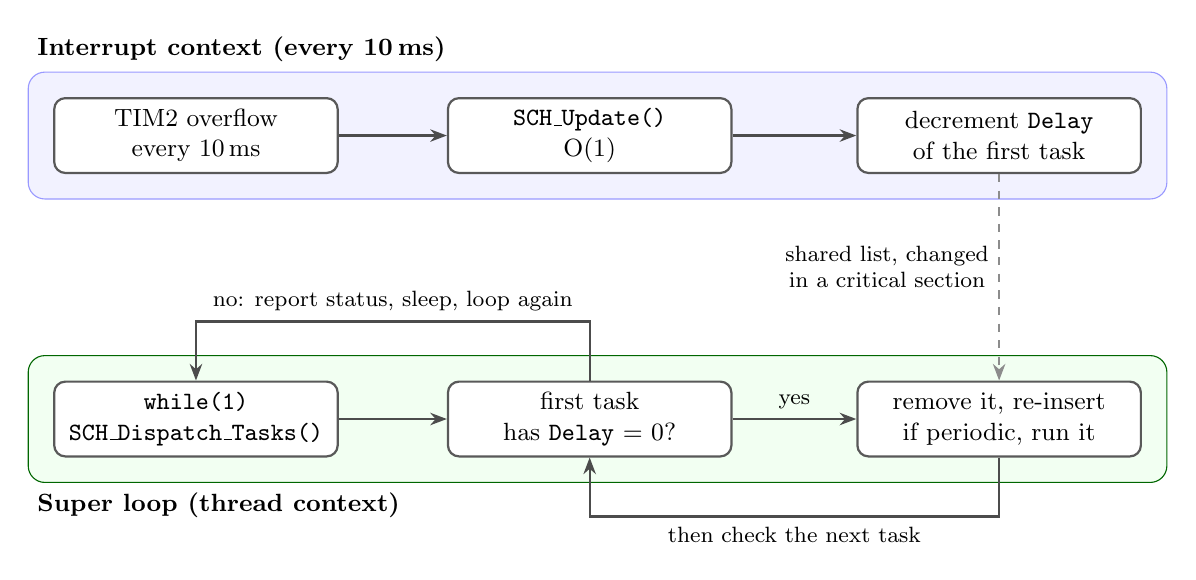
\begin{tikzpicture}[
  bx/.style={draw=black!65, rounded corners=4pt, line width=0.8pt, fill=white, align=center, font=\small, minimum width=3.6cm, minimum height=0.95cm},
  ar/.style={-{Stealth[length=6pt]}, line width=0.8pt, draw=black!70},
  lb/.style={font=\footnotesize, align=center}]
\node[bx] (t)  at (0,0)    {TIM2 overflow\\ every 10\,ms};
\node[bx] (u)  at (5,0)    {\code{SCH\_Update()}\\ O(1)};
\node[bx] (h)  at (10.2,0) {decrement \code{Delay}\\ of the first task};
\node[bx] (d)  at (0,-3.6)   {\code{while(1)}\\ \code{SCH\_Dispatch\_Tasks()}};
\node[bx] (c)  at (5,-3.6)   {first task\\ has \code{Delay} = 0?};
\node[bx] (r)  at (10.2,-3.6){remove it, re-insert\\ if periodic, run it};
\begin{scope}[on background layer]
\node[fit=(t)(u)(h), inner sep=9pt, fill=blue!5, draw=blue!40, rounded corners=6pt, label={[font=\small\bfseries, anchor=south west]north west:Interrupt context (every 10\,ms)}] {};
\node[fit=(d)(c)(r), inner sep=9pt, fill=green!5, draw=green!40!black, rounded corners=6pt, label={[font=\small\bfseries, anchor=north west]south west:Super loop (thread context)}] {};
\end{scope}
\draw[ar] (t) -- (u);
\draw[ar] (u) -- (h);
\draw[ar] (d) -- (c);
\draw[ar] (c) -- node[above,lb]{yes} (r);
\draw[ar] (r.south) -- ++(0,-0.75) -| node[pos=0.25,below,lb]{then check the next task} (c.south);
\draw[ar] (c.north) -- ++(0,0.75) -| node[pos=0.25,above,lb]{no: report status, sleep, loop again} (d.north);
\draw[ar, dashed, draw=black!45] (h.south) -- node[left,lb,pos=0.45]{shared list, changed\\ in a critical section} (r.north);
\end{tikzpicture}
\caption{The interrupt only counts time; the super loop runs the tasks}
\label{fig:flow}
\end{figure}

\subsection{Data structure: a sorted delta list}
\label{sec:ds}
The scheduler in the manual keeps the tasks in an array, and \code{SCH\_Update()} visits every slot of the array at each tick. This is the ``O(n) search in the \code{SCH\_Update} function'' that the manual lists as unsatisfactory. This project keeps the same static array \code{SCH\_tasks\_G[]}, but links the used slots into a list \emph{sorted by the time they are due}. Each task does not store the time until it runs, but only the number of ticks \emph{after the task in front of it} (a ``delta list''). For example, tasks due in 50, 80, 80 and 200 ticks are stored as in Figure~\ref{fig:delta}.

\begin{figure}[H]
\centering
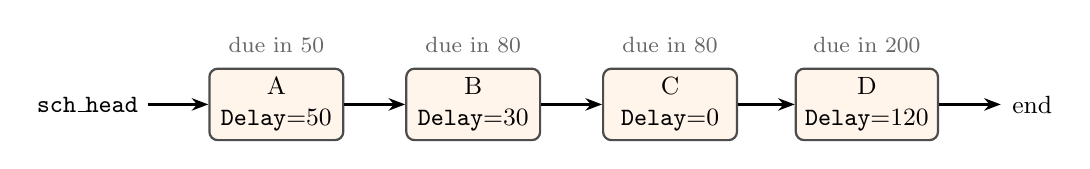
\begin{tikzpicture}[
  nd/.style={draw=black!70, line width=0.8pt, rounded corners=3pt, minimum width=1.7cm, minimum height=0.9cm, align=center, font=\small, fill=orange!8},
  ar/.style={-{Stealth[length=6pt]}, line width=0.8pt}]
\node[font=\small\ttfamily] (hd) at (0,0) {sch\_head};
\node[nd] (a) at (2.4,0) {A\\ \code{Delay}=50};
\node[nd] (b) at (4.9,0) {B\\ \code{Delay}=30};
\node[nd] (c) at (7.4,0) {C\\ \code{Delay}=0};
\node[nd] (d) at (9.9,0) {D\\ \code{Delay}=120};
\node[font=\small] at (12.0,0) {end};
\draw[ar] (hd) -- (a); \draw[ar] (a) -- (b); \draw[ar] (b) -- (c); \draw[ar] (c) -- (d); \draw[ar] (d) -- (11.6,0);
\foreach \n/\t in {a/50, b/80, c/80, d/200} \node[font=\footnotesize, black!60, above=2pt of \n] {due in \t};
\end{tikzpicture}
\caption{The waiting list: each \code{Delay} is relative to the previous task}
\label{fig:delta}
\end{figure}

With this structure, one tick for \emph{all} tasks is a single decrement on the first task. A second list, the free list, links the empty slots, so \code{SCH\_Add\_Task()} also finds a slot without searching.

\src{scheduler.c}{51}{68}{The task structure and the scheduler variables}

Compared with the structure of the manual (Program 1.7):
\begin{itemize}[leftmargin=1.4em,itemsep=1pt]
\item \code{RunMe} is not needed: a task that is due is always the first task of the list with \code{Delay == 0}, so its position is the flag.
\item \code{Next} is new: the index of the next task in the list (an array index, not a pointer, so it is only 1 byte).
\item \code{TaskID} is a real ID (1, 2, 3, \ldots), not the position in the array. When a slot is reused, the new task gets a new ID, so an old ID can never delete the wrong task.
\end{itemize}
A task uses $4 + 3\times4 + 1 = 17$ bytes of data (20 bytes with the alignment of the ARM compiler), the same budget as the scheduler of the manual.

\subsection{\code{SCH\_Update()}: O(1)}
\label{sec:update}
The function has no loop. It increases the time counter used by \code{get\_time()} and decrements the \code{Delay} of the first task. When that \code{Delay} is already 0, the task is due but the dispatcher has not taken it yet (another task is running); the tick is then saved in \code{sch\_late\_ticks} so that it is not lost (Section~\ref{sec:late}).
\src{scheduler.c}{150}{161}{\code{SCH\_Update()}}

\subsection{\code{SCH\_Add\_Task()}: sorted insert}
\label{sec:add}
The work that \code{SCH\_Update()} does not do is moved here, outside the interrupt. \code{SCH\_Insert()} walks the list, subtracting the \code{Delay} of every task it passes, until it finds the place of the new task. The task behind the new one gets the new \code{Delay} subtracted from its own, so its due time does not change. Tasks due at the same tick are kept in the order they were added (smaller ID first), which is also the order of the array scan in the manual. This walk is O(n), but it runs in the super loop, never in the interrupt.
\src{scheduler.c}{74}{101}{Inserting a task into the sorted list}

\code{SCH\_Add\_Task()} takes a slot from the free list, gives it the next ID and inserts it. When the array is full, it returns \code{NO\_TASK\_ID}, which is 0, and sets the error code \code{ERROR\_SCH\_TOO\_MANY\_TASKS}, as required by Section 2.3.2 of the manual.
\src{scheduler.c}{163}{196}{\code{SCH\_Add\_Task()}}

\subsection{\code{SCH\_Dispatch\_Tasks()}}
As long as the first task has \code{Delay == 0}, the dispatcher removes it from the list. A periodic task is inserted again \emph{before} it runs, one \code{Period} after the time it was due. The next run is therefore counted from the planned time, not from the time the task finishes, so the period does not drift. A one-shot task gives its slot back to the free list. The task itself is called outside the critical section, with interrupts enabled, so ticks keep being counted while it runs.
\src{scheduler.c}{231}{263}{\code{SCH\_Dispatch\_Tasks()}}

\subsection{\code{SCH\_Delete\_Task()}}
\label{sec:delete}
The task is searched by its ID (O(n), in the super loop). When it is removed, its \code{Delay} is added to the next task, so the remaining tasks keep their due times. Deleting an ID that does not exist returns \code{RETURN\_ERROR} and sets \code{ERROR\_SCH\_CANNOT\_DELETE\_TASK}.
\src{scheduler.c}{198}{229}{\code{SCH\_Delete\_Task()}}

\subsection{Shared data and late ticks}
\label{sec:late}
The list is changed in the super loop and read by the interrupt. A tick that arrived in the middle of an insert would decrement the wrong task, so every change of the list is done in a short critical section. The macros save PRIMASK and restore it afterwards (instead of a plain enable), so they also work if they are ever called with interrupts already disabled. These are the only hardware-dependent lines of the scheduler; on a PC they are empty, which is how the unit tests are built (Section~\ref{sec:test}).
\src{scheduler.c}{38}{47}{Port section}

If a task runs longer than one tick while the next task is already due, \code{SCH\_Update()} cannot decrement a \code{Delay} of 0. Ignoring the tick would delay every following task for ever. The tick is kept in \code{sch\_late\_ticks} and paid back to the new first task as soon as the due task has left the list. \code{SCH\_Add\_Task()} also adds these ticks to the \code{DELAY} of a task added at that moment, so that the delay counts from \emph{now}.
\src{scheduler.c}{113}{128}{Paying back the late ticks}

\subsection{\code{get\_time()}, error report and sleep}
\code{get\_time()} returns the tick counter multiplied by \code{SCH\_TICK\_MS}, so the timestamps are exact to one tick (10\,ms), as the demonstration requires. \code{SCH\_Report\_Status()} reports a new error code once, through \code{SCH\_Error\_Callback()}. The default callback is a weak empty function (the same idea as the HAL callbacks); \code{tasks.c} replaces it with one that prints \code{ERROR <code>} on the terminal. The optional sleep of Section 2.3.8 is implemented with \code{\_\_WFI()} but is disabled by default (\code{SCH\_SLEEP\_ENABLED = 0}). The optional watchdog of Section 2.3.10 is not implemented.
\src{scheduler.c}{265}{291}{\code{get\_time()}, error report and sleep}

\subsection{Cost of each function}
\begin{center}\small
\begin{tabular}{llll}
\toprule
\textbf{Function} & \textbf{Called from} & \textbf{Cost} & \textbf{Manual (array scan)}\\
\midrule
\code{SCH\_Update()} & TIM2 interrupt & O(1) & O(n) every tick\\
\code{SCH\_Add\_Task()} & super loop, tasks & O(n) sorted insert & O(n) search for a gap\\
\code{SCH\_Delete\_Task()} & super loop, tasks & O(n) search by ID & O(1) by index\\
\code{SCH\_Dispatch\_Tasks()} & super loop & O(n) per task run & O(n) scan\\
\code{get\_time()} & anywhere & O(1) & --\\
\bottomrule
\end{tabular}
\end{center}
The cost is moved from the interrupt, which runs 100 times per second, to adding and deleting, which happen rarely.

% ======================= APPLICATION =======================
\section{Demonstration program}
\label{sec:app}
\report{Registering the tasks}
\code{main()} initialises the scheduler and registers ten tasks before entering the loop. The one-shot tasks are added in the order C, A, B on purpose: they must still be called in the order A, B, C. Their delays (250\,ms and more) are much longer than the time needed to reach the loop. TIM2 is started last, so time 0 of the scheduler is the moment the loop begins. The super loop only calls the dispatcher.
\src{main.c}{98}{136}{Task registration and the super loop}

\begin{center}
\small
\begin{tabularx}{\linewidth}{>{\ttfamily}l l l X}
\toprule
\normalfont\textbf{Task} & \textbf{First run} & \textbf{Period} & \textbf{Action}\\
\midrule
task\_led1 & 0 & 0.5\,s & \multirow{5}{=}{toggle \code{LED\_1} \ldots{} \code{LED\_5}, print the time}\\
task\_led2 & 0 & 1\,s & \\
task\_led3 & 0 & 1.5\,s & \\
task\_led4 & 0 & 2\,s & \\
task\_led5 & 0 & 2.5\,s & \\
task\_tick & 0 & 10\,ms & print the time; deleted at 1\,s\\
task\_once\_a/\_b/\_c & 250/750/1250\,ms & one-shot & print the time\\
task\_stop\_tick & 1000\,ms & one-shot & \code{SCH\_Delete\_Task()} on \code{task\_tick}\\
\bottomrule
\end{tabularx}
\end{center}
The 10\,ms task prints 100 lines per second, so it is deleted after one second to keep the terminal readable. This also demonstrates \code{SCH\_Delete\_Task()}.

\report{The tasks}
Every task prints one line \code{<time in ms> <name>} on USART1, where the time is \code{get\_time()} at the moment the task starts. \code{printf()} is not used because it is large and slow on this small MCU; the line is built in a buffer and sent with one \code{HAL\_UART\_Transmit()}.
\src{tasks.c}{28}{55}{Printing a timestamp and the first LED task}
\src{tasks.c}{77}{103}{The 10\,ms task, the one-shot tasks and the delete task}

\report{Proteus schematic}
The schematic (Figure~\ref{fig:run}) contains the STM32F103C6 loaded with \code{Lab4.hex}, five LEDs and a Virtual Terminal. Each LED has its anode at +3.3\,V and its cathode on a pin of PA11--PA15. The terminal input RXD is connected to PA9 (USART1\_TX) through a net label, and set to 57600 baud, 8 data bits, no parity, 1 stop bit, the same as \code{huart1}. The schematic reuses the one of Lab 3, so the net labels keep their Lab 3 names; the table gives the mapping.
\begin{center}
\begin{tabular}{l l l l l}
\toprule
\textbf{Task} & \textbf{Period} & \textbf{Pin} & \textbf{Net label} & \textbf{LED}\\
\midrule
\code{task\_led1} & 0.5\,s & PA11 & \code{LED\_AMBER\_1} & D10\\
\code{task\_led2} & 1\,s   & PA12 & \code{LED\_GREEN\_1} & D14\\
\code{task\_led3} & 1.5\,s & PA13 & \code{LED\_RED\_2}   & D7\\
\code{task\_led4} & 2\,s   & PA14 & \code{LED\_AMBER\_2} & D12\\
\code{task\_led5} & 2.5\,s & PA15 & \code{LED\_GREEN\_2} & D11\\
\midrule
UART output & -- & PA9 & \code{EN3} & Virtual Terminal (RXD)\\
\bottomrule
\end{tabular}
\end{center}

% ======================= RESULTS =======================
\section{Results}
\report{The first 2.5 seconds}
Listing~\ref{lst:trace} is the beginning of the output. The 101 lines \code{0 TICK}, \code{10 TICK}, \ldots, \code{1000 TICK} are left out (the dots); they are 10\,ms apart, which shows the 10\,ms callback and that \code{get\_time()} is accurate to 10\,ms.

\begin{lstlisting}[style=term, caption={Output of the first 2.5\,s (TICK lines left out)}, label={lst:trace}]
Lab 4 - cooperative scheduler, tick = 10 ms
0 LED1
0 LED2
0 LED3
0 LED4
0 LED5
0 TICK
10 TICK
...           (one TICK line every 10 ms)
250 TICK
250 ONCE-A
...
500 LED1
...
750 ONCE-B
...
1000 LED1
1000 LED2
1000 TICK
1000 TICK deleted
1250 ONCE-C
1500 LED1
1500 LED3
2000 LED1
2000 LED2
2000 LED4
2500 LED1
2500 LED5
\end{lstlisting}
\begin{itemize}[leftmargin=1.4em,itemsep=1pt]
\item \textbf{Order of the one-shot tasks.} They were added in the order C, A, B, but are called at 250, 750 and 1250\,ms in the order A, B, C: callbacks are delivered by time, not by order of adding.
\item \textbf{Several timeouts at once.} At 1000\,ms four tasks are due in the same tick, and all of them run, in the order they were added.
\item \textbf{Delete.} After \code{1000 TICK deleted} there is no more \code{TICK} line.
\end{itemize}

\report{Simulation in Proteus}
Figure~\ref{fig:run} is the simulation between 7000 and 7500\,ms. The timestamps on the terminal are exact multiples of the periods:
\begin{center}
\begin{tabular}{l l l l}
\toprule
\textbf{Task} & \textbf{Period} & \textbf{Times on the terminal (ms)} & \textbf{Interval}\\
\midrule
LED1 & 500\,ms  & 4500, 5000, 5500, 6000, 6500, 7000 & 500\\
LED2 & 1000\,ms & 4000, 5000, 6000, 7000 & 1000\\
LED3 & 1500\,ms & 4500, 6000 & 1500\\
LED4 & 2000\,ms & 4000, 6000 & 2000\\
LED5 & 2500\,ms & 5000 & next: 7500\\
\bottomrule
\end{tabular}
\end{center}

\begin{figure}[H]
\centering
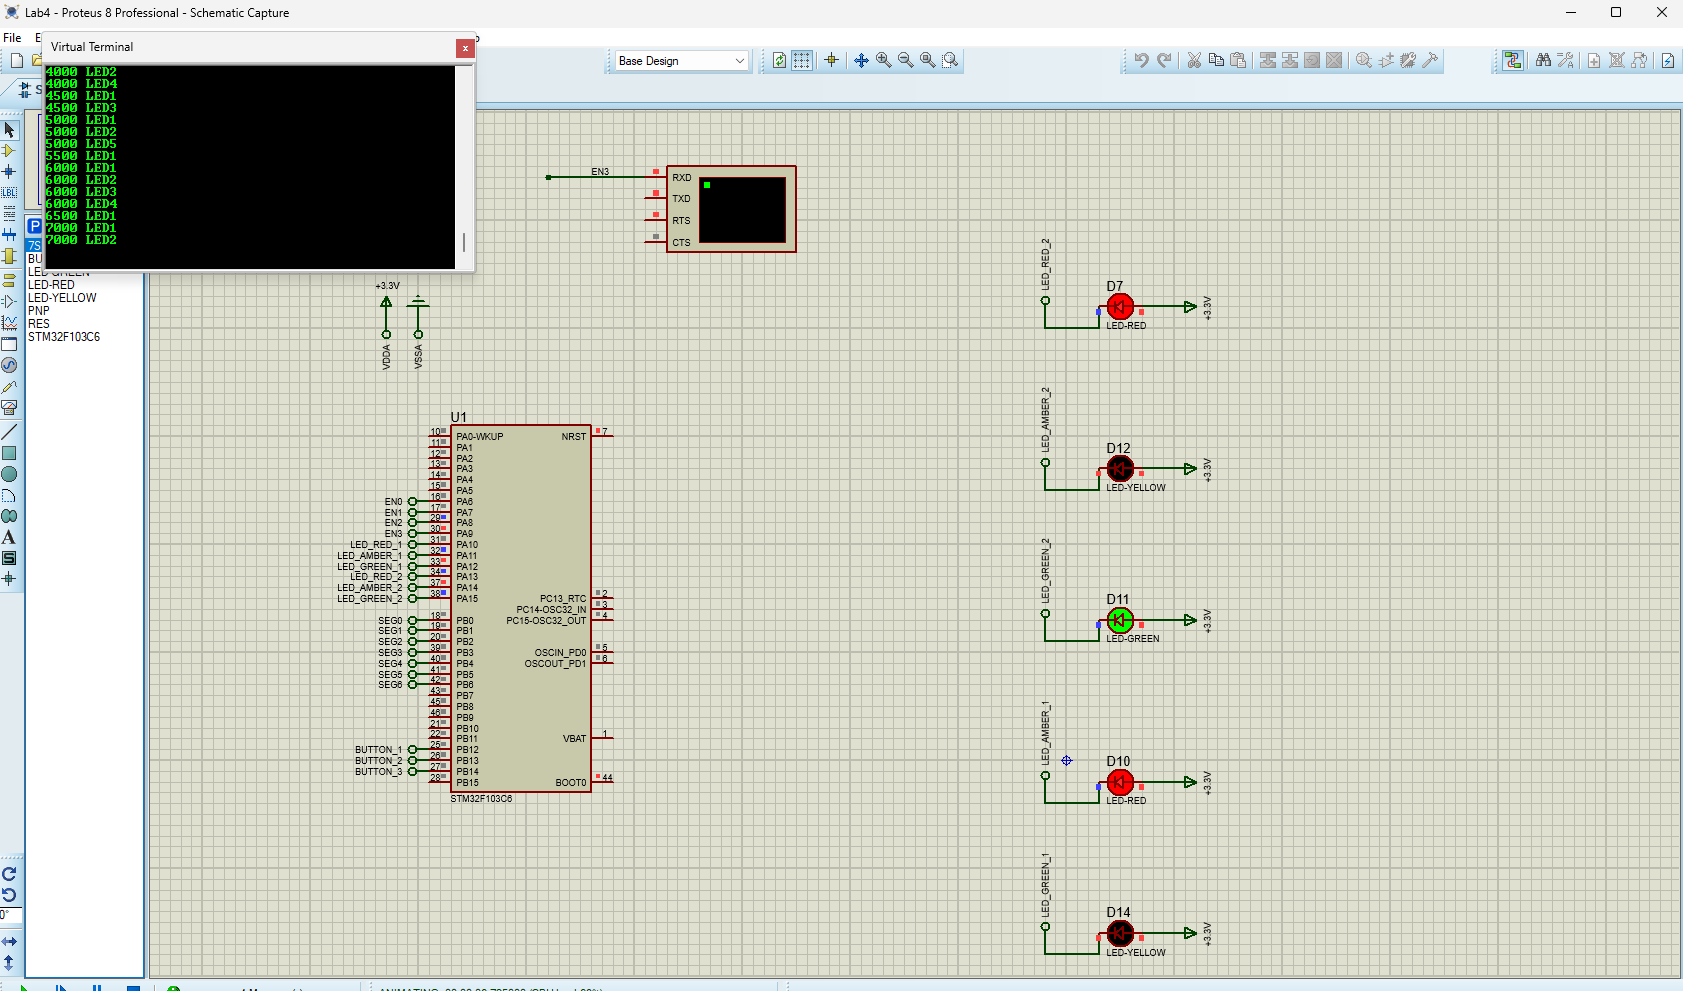
\includegraphics[width=\linewidth]{proteus_run}\\[6pt]
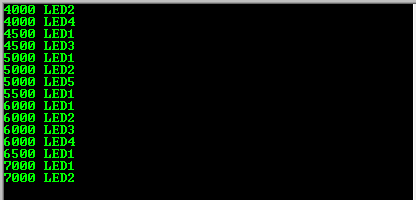
\includegraphics[height=5.6cm]{proteus_terminal}\hspace{1.2cm}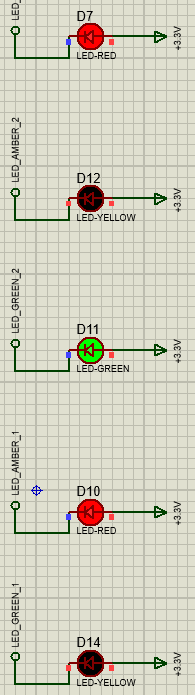
\includegraphics[height=5.6cm]{proteus_leds}
\caption{Proteus simulation between 7000 and 7500\,ms. Bottom: the Virtual Terminal and the LED column enlarged. D7, D11 and D10 are on; D12 and D14 are off}
\label{fig:run}
\end{figure}

\report{LED states}
Each run of an LED task toggles its pin. The first run at 0\,ms pulls the pin LOW, so the LED turns on; an LED is therefore on after an odd number of runs (Figure~\ref{fig:wave}). Note that a task period of 0.5\,s gives an LED that is on for 0.5\,s and off for 0.5\,s.

At the moment of Figure~\ref{fig:run} (between 7000 and 7500\,ms), LED1 has run 15 times (0, 500, \ldots, 7000), LED2 8 times, LED3 5 times (0, 1500, 3000, 4500, 6000), LED4 4 times and LED5 3 times (0, 2500, 5000). So LED1, LED3 and LED5 (D10, D7, D11) are on, and LED2 and LED4 (D14, D12) are off, which is what the screenshot shows.

\begin{figure}[H]
\centering
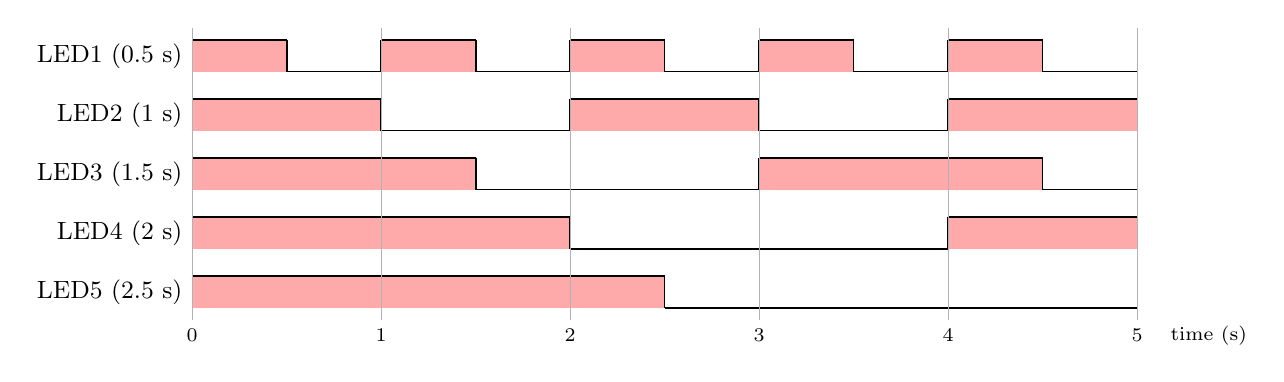
\begin{tikzpicture}
\fill[ledon] (0.000,0.00) rectangle (1.200,-0.40);
\draw[line width=0.6pt] (0.000,0.00) -- (1.200,0.00);
\draw[line width=0.6pt] (1.200,0.00) -- (1.200,-0.40);
\draw[line width=0.6pt] (1.200,-0.40) -- (2.400,-0.40);
\draw[line width=0.6pt] (2.400,0.00) -- (2.400,-0.40);
\fill[ledon] (2.400,0.00) rectangle (3.600,-0.40);
\draw[line width=0.6pt] (2.400,0.00) -- (3.600,0.00);
\draw[line width=0.6pt] (3.600,0.00) -- (3.600,-0.40);
\draw[line width=0.6pt] (3.600,-0.40) -- (4.800,-0.40);
\draw[line width=0.6pt] (4.800,0.00) -- (4.800,-0.40);
\fill[ledon] (4.800,0.00) rectangle (6.000,-0.40);
\draw[line width=0.6pt] (4.800,0.00) -- (6.000,0.00);
\draw[line width=0.6pt] (6.000,0.00) -- (6.000,-0.40);
\draw[line width=0.6pt] (6.000,-0.40) -- (7.200,-0.40);
\draw[line width=0.6pt] (7.200,0.00) -- (7.200,-0.40);
\fill[ledon] (7.200,0.00) rectangle (8.400,-0.40);
\draw[line width=0.6pt] (7.200,0.00) -- (8.400,0.00);
\draw[line width=0.6pt] (8.400,0.00) -- (8.400,-0.40);
\draw[line width=0.6pt] (8.400,-0.40) -- (9.600,-0.40);
\draw[line width=0.6pt] (9.600,0.00) -- (9.600,-0.40);
\fill[ledon] (9.600,0.00) rectangle (10.800,-0.40);
\draw[line width=0.6pt] (9.600,0.00) -- (10.800,0.00);
\draw[line width=0.6pt] (10.800,0.00) -- (10.800,-0.40);
\draw[line width=0.6pt] (10.800,-0.40) -- (12.000,-0.40);
\node[left,font=\small] at (0,-0.20) {LED1 (0.5 s)};
\fill[ledon] (0.000,-0.75) rectangle (2.400,-1.15);
\draw[line width=0.6pt] (0.000,-0.75) -- (2.400,-0.75);
\draw[line width=0.6pt] (2.400,-0.75) -- (2.400,-1.15);
\draw[line width=0.6pt] (2.400,-1.15) -- (4.800,-1.15);
\draw[line width=0.6pt] (4.800,-0.75) -- (4.800,-1.15);
\fill[ledon] (4.800,-0.75) rectangle (7.200,-1.15);
\draw[line width=0.6pt] (4.800,-0.75) -- (7.200,-0.75);
\draw[line width=0.6pt] (7.200,-0.75) -- (7.200,-1.15);
\draw[line width=0.6pt] (7.200,-1.15) -- (9.600,-1.15);
\draw[line width=0.6pt] (9.600,-0.75) -- (9.600,-1.15);
\fill[ledon] (9.600,-0.75) rectangle (12.000,-1.15);
\draw[line width=0.6pt] (9.600,-0.75) -- (12.000,-0.75);
\node[left,font=\small] at (0,-0.95) {LED2 (1 s)};
\fill[ledon] (0.000,-1.50) rectangle (3.600,-1.90);
\draw[line width=0.6pt] (0.000,-1.50) -- (3.600,-1.50);
\draw[line width=0.6pt] (3.600,-1.50) -- (3.600,-1.90);
\draw[line width=0.6pt] (3.600,-1.90) -- (7.200,-1.90);
\draw[line width=0.6pt] (7.200,-1.50) -- (7.200,-1.90);
\fill[ledon] (7.200,-1.50) rectangle (10.800,-1.90);
\draw[line width=0.6pt] (7.200,-1.50) -- (10.800,-1.50);
\draw[line width=0.6pt] (10.800,-1.50) -- (10.800,-1.90);
\draw[line width=0.6pt] (10.800,-1.90) -- (12.000,-1.90);
\node[left,font=\small] at (0,-1.70) {LED3 (1.5 s)};
\fill[ledon] (0.000,-2.25) rectangle (4.800,-2.65);
\draw[line width=0.6pt] (0.000,-2.25) -- (4.800,-2.25);
\draw[line width=0.6pt] (4.800,-2.25) -- (4.800,-2.65);
\draw[line width=0.6pt] (4.800,-2.65) -- (9.600,-2.65);
\draw[line width=0.6pt] (9.600,-2.25) -- (9.600,-2.65);
\fill[ledon] (9.600,-2.25) rectangle (12.000,-2.65);
\draw[line width=0.6pt] (9.600,-2.25) -- (12.000,-2.25);
\node[left,font=\small] at (0,-2.45) {LED4 (2 s)};
\fill[ledon] (0.000,-3.00) rectangle (6.000,-3.40);
\draw[line width=0.6pt] (0.000,-3.00) -- (6.000,-3.00);
\draw[line width=0.6pt] (6.000,-3.00) -- (6.000,-3.40);
\draw[line width=0.6pt] (6.000,-3.40) -- (12.000,-3.40);
\node[left,font=\small] at (0,-3.20) {LED5 (2.5 s)};
\foreach \s in {0,...,5} {\draw[black!30] (\s*2.4,0.15) -- (\s*2.4,-3.55); \node[font=\scriptsize, below] at (\s*2.4,-3.55) {\s};}
\node[font=\scriptsize, anchor=west] at (12.3,-3.75) {time (s)};
\end{tikzpicture}
\caption{LED states during the first 5\,s (shaded = pin LOW = LED on)}
\label{fig:wave}
\end{figure}

\report{Timing budget of the tasks}
At 57600 baud one character takes $10/57600 = 0.174$\,ms, so a line such as \code{1000 LED1} (11 characters with \code{\textbackslash r\textbackslash n}) takes about 1.9\,ms. \code{HAL\_UART\_Transmit()} waits until the line is sent, so this is the duration of an LED task. The busiest ticks are at 1000\,ms (four lines, about 9\,ms) and every 30\,s, when all five LED tasks are due together (five lines of 12 characters, about 10.4\,ms). In the second case the next tick arrives while the last task is still printing. This is not a problem: the tick is counted by the interrupt, and the tasks that just ran were already re-inserted, so the next runs keep their exact times. The case of a task that really runs for several ticks is checked by the unit tests below.

% ======================= TESTS =======================
\section{Unit tests}
\label{sec:test}
The scheduler has no hardware dependency apart from the port section (Section~\ref{sec:late}), so \code{scheduler.c} is also compiled on a PC with \code{-DSCH\_HOST\_TEST}. \code{test/test\_scheduler.c} calls \code{SCH\_Update()} by hand to simulate the ticks and checks:
\begin{itemize}[leftmargin=1.4em,itemsep=1pt]
\item the five periods 0.5--2.5\,s over 60\,s: every run at exactly $k \times$ period, in time order, ties in the order of adding;
\item one-shot tasks added in the wrong order are run in the right order, at the right time;
\item \code{SCH\_Delete\_Task()}: deleting a task does not move the others; an unknown or old ID is refused;
\item a full array: the 41st task is refused with \code{ERROR\_SCH\_TOO\_MANY\_TASKS}, and a slot can be reused after a delete;
\item a task that runs for more than 3 ticks: the other tasks are late by at most that time and no run is lost;
\item a random test: 200 random scenarios of 20000 ticks, where tasks add and delete other tasks and sometimes run for several ticks. A second, very simple model of the scheduler (absolute times, full search) runs next to the real one, and every task started by the scheduler must be the one the model expects, at the tick the model expects.
\end{itemize}

\begin{lstlisting}[style=term, caption={Building and running the unit tests}]
$ cd test
$ gcc -Wall -Wextra -DSCH_HOST_TEST -I../stm32/Core/Inc test_scheduler.c \
      ../stm32/Core/Src/scheduler.c -o test_scheduler
$ ./test_scheduler
test: five periodic tasks 0.5 s .. 2.5 s for 60 s
test: one-shot tasks added in the wrong order
test: SCH_Delete_Task
test: more than SCH_MAX_TASKS tasks
test: a task that runs for 35 ms does not shift the other tasks
test: random, compared with the reference model
  15200747 task runs checked, 1795442 tasks added, 1279026 deleted, 348129 refused (array full)

ALL TESTS PASSED
\end{lstlisting}

% ======================= DISCUSSION =======================
\section{Discussion}
\report{The 10\,Hz limit in the manual}
Among the unsatisfactory designs, the manual lists ``interrupt frequencies greater than 10\,Hz, if your timer ticks regularly''. The same section asks for ``a regular 10\,ms timer tick'' (100\,Hz) and timestamps accurate to 10\,ms, which a 10\,Hz tick cannot give. This project follows the explicit demonstration requirement and uses a 10\,ms tick. The cost of this rate is kept low because each interrupt is O(1). A design that respected both points would be a tickless scheduler, which programs the timer to interrupt only when the first task of the list is due; the sorted delta list used here is the data structure such a design needs.

\report{Limitations}
\begin{itemize}[leftmargin=1.4em,itemsep=1pt]
\item The scheduler is cooperative: a task that never returns blocks all others. The tasks must stay short (here, under one tick).
\item \code{get\_time()} is exact to one tick only, and wraps after $2^{32}$ ticks (about 497 days).
\item The watchdog (Section 2.3.10) is not implemented, and the sleep mode is present but disabled.
\end{itemize}

\ifdefempty{\videolink}{}{%
\report{Demonstration video}
The video of the simulation is available at:
\begin{center}\expandafter\url\expandafter{\videolink}\end{center}
}

\end{document}
